\subsection{Hyperparamters}

Through grid search the best combination of $\lambda$- and degree-values where found to be: 

\begin{table}[h!]
    \centering
    \begin{tabular}{|c|c|c|c|}
        \hline
        & & \textbf{Franke Function} & \textbf{Terrain Data} \\ \hline
        \textbf{Ridge} & $\lambda$ & 2.4 $\times 10^{-2}$ & 3.0 $\times 10^{-5}$ \\ 
         & degree & 7 & 4 \\ \hline
        \textbf{Lasso} & $\lambda$ & 1.7 $\times 10^{-5}$ & 2.2 $\times 10^{-4}$ \\ 
         & degree & 7 & 6 \\ \hline
    \end{tabular}
    \caption{Best pairs of $\lambda$- and degree values found through grid search}
    \label{tab:grid}
\end{table}

\mia{do these need a discussion?}

\subsection{Franke function}

\mia{fix titles in plots so that they do not overlap with the captions, maybe also change the xlabel to "degree of complexity/polynomial" or smt}

\begin{figure}[h!]
    \centering
    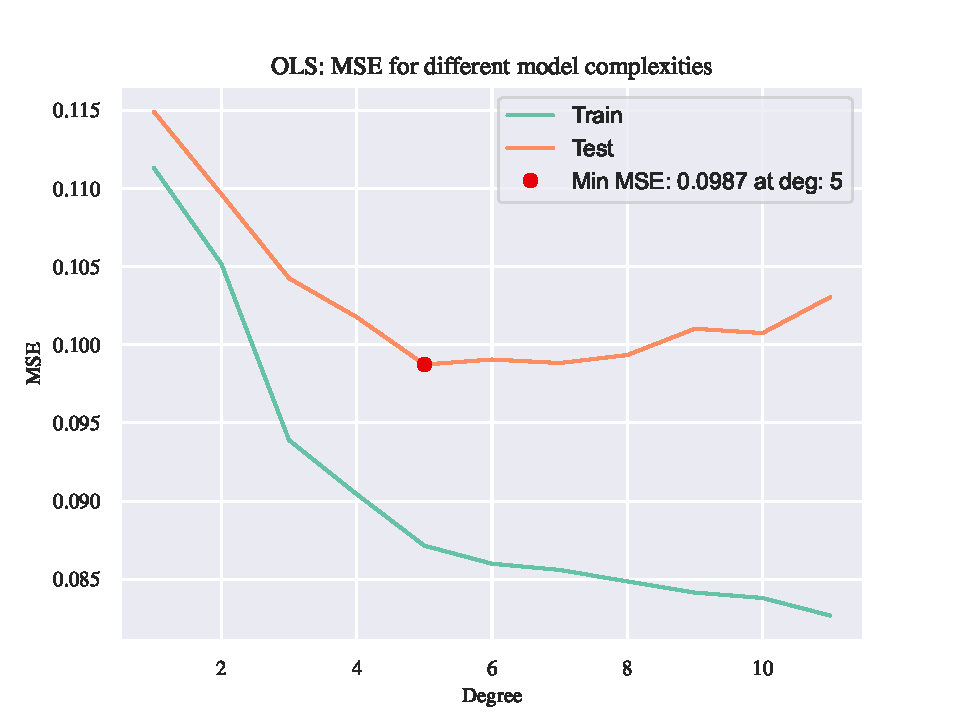
\includegraphics[width=1\linewidth]{project_1_alt/figures/figures_in_report/OLS_MSE_Franke_Noise.pdf}
    \caption{Mean squared error (MSE) for the ordinary least squares model both on training- and test data.}
    \label{fig:mseols}
\end{figure}

Fig. \ref{fig:mseols} shows how the error initially decreases as the degree of complexity increases. This seems reasonable as the Franke function makes up a complicated surface and one would think that higher degree polynomials are necessary to replicate it. 

We furthermore notice how the test error reaches its minimum at deg = 5. The test error increases as the polynomial degree further increased. We use the test error to choose the optimal degree of complexity. The training error continues to decrease. This is due to overfitting and the fact that OLS is designed to minimize the MSE. We use this as a sanity check of our model implementation.

\begin{figure}[h!]
    \centering
    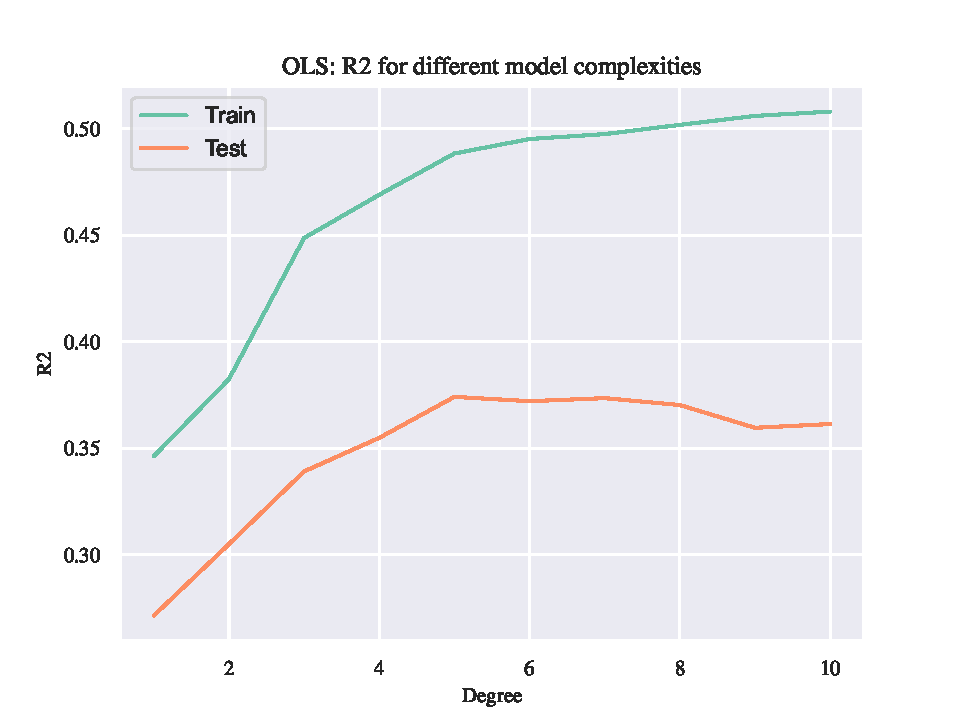
\includegraphics[width=1\linewidth]{project_1_alt/figures/figures_in_report/OLS_R2_Franke_Noise.pdf}
    \caption{$R^2$ for the ordinary least squares model both on training- and test data.}
    \label{fig:r2ols}
\end{figure}

The $R^2$ value increases as higher degree polynomials are introduced to the ordinary least squares model, as shown in Fig. \ref{fig:r2ols}. This is reasonable as we likely need higher degree polynomials to explain more variance in the data. The increase in $R^2$ halters at around degree equal to 10. At this point, introducing higher degree polynoimals does not help explain further variance in the data. The value of $R^2$ for the test data is lower then the one for the training data. This might be a sign that the model does not generalize well. 

\begin{figure}[h!]
    \centering
    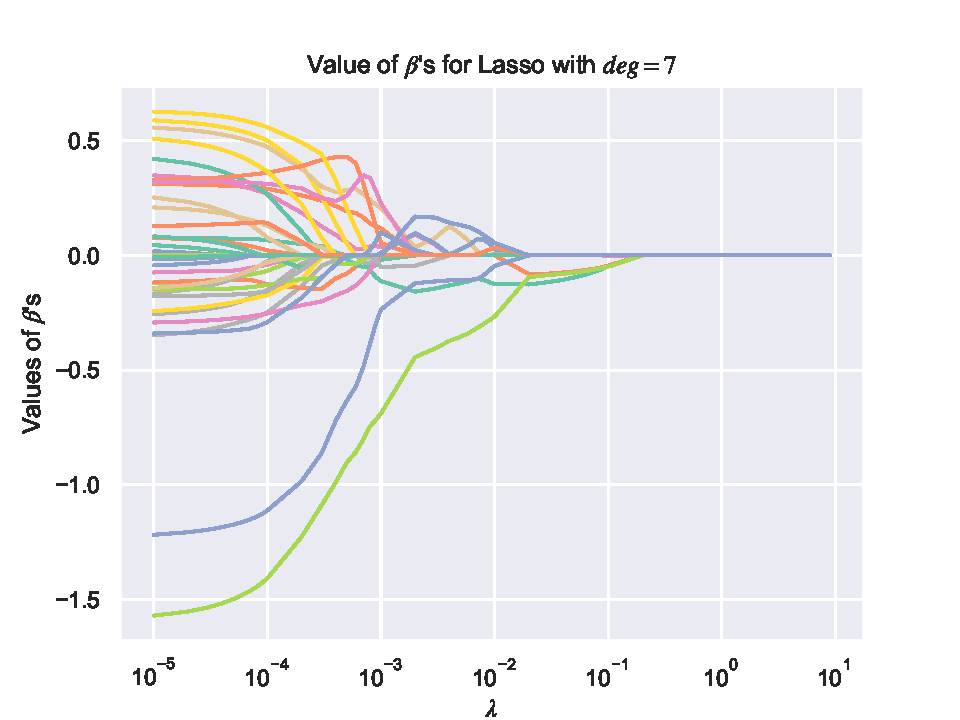
\includegraphics[width=1\linewidth]{project_1_alt/figures/figures_in_report/Ridge_Betas_lambda_Franke_Noise_const_deg.pdf}
    \caption{The values of the parameters $\beta$ for the ridge regression model with polynomials up to a degree of seven for increasing values of $\lambda$. Each colored line represents one $\beta_j$.}
    \label{fig:ridge_betas}
\end{figure}

\begin{figure}[h!]
    \centering
    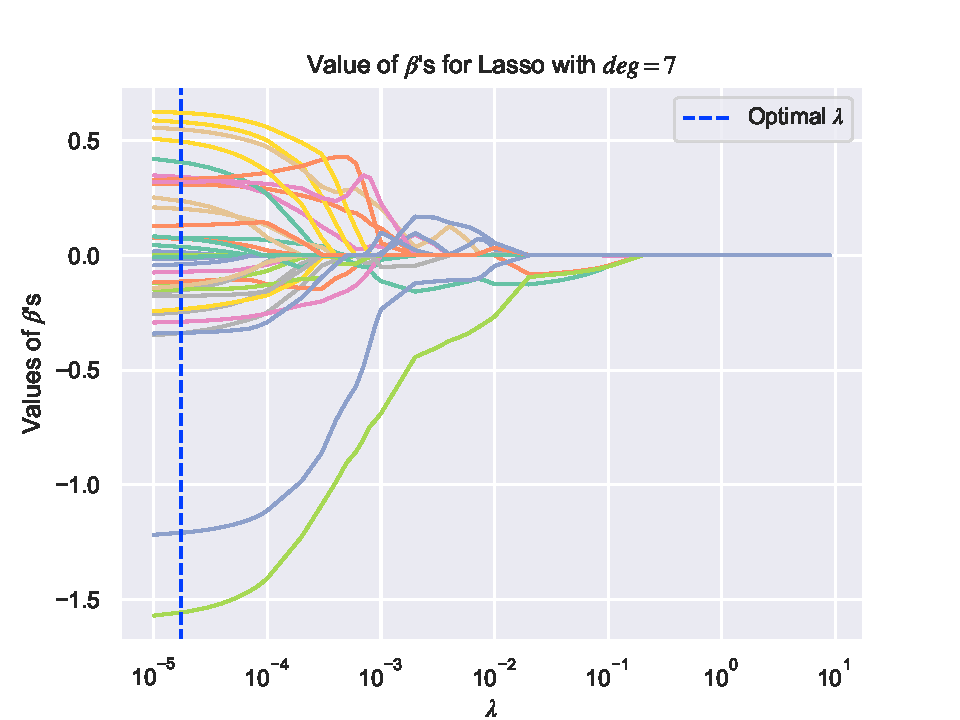
\includegraphics[width=1\linewidth]{project_1_alt/figures/figures_in_report/lasso_Betas_lambda_Franke_Noise_const_deg.pdf}
    \caption{The values of the parameters $\beta$ for the lasso regression model with polynomials up to a degree of seven for increasing values of $\lambda$. Each colored line represents one $\beta_j$.}
    \label{fig:lasso_betas}
\end{figure}

The $\beta$'s values for our Ridge- and Lasso regression models are presented in Fig. \ref{fig:ridge_betas} and Fig. \ref{fig:lasso_betas} respectfully. For both models, we observe that the values of the coefficients are forced towards zero, and thereby also each other, as the penalty increases. For the Ridge regression coefficients, all have non-zero values regardless of the size of the penalty. For Lasso regression however, we observe that some are brought to zero at a sufficiently large penalty. Closer to $\lambda = 10^0 = 1$ all values of the $\beta$'s are brought to zero. A $\lambda$ value of this size seems highly unreasonable. The vertical line in each plot shows the optimal $\lambda$ in combination with the degree of complexity found through the grid search (numbers are available in Tab. \ref{tab:grid}). \mia{implications}

\begin{figure}
    \centering
    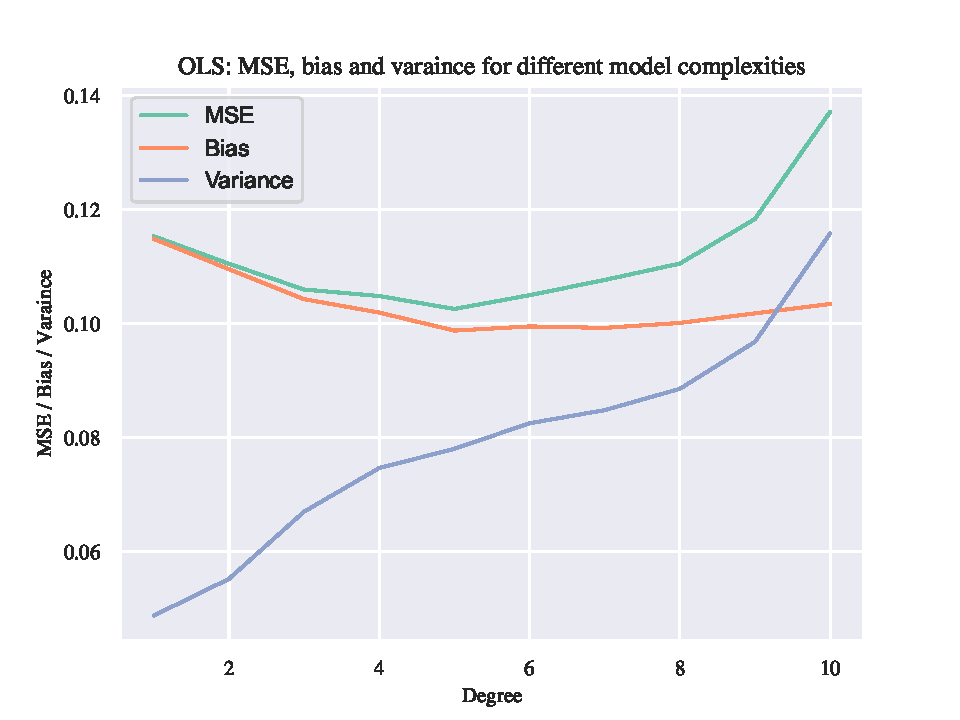
\includegraphics[width=1\linewidth]{project_1_alt/figures/figures_in_report/bias_var_Franke_Noise_bootstrap.pdf}
    \caption{MSE decomposed into a bias and a variance term for an ordinary least squares model trained with bootstrapping. \mia{must find minimum and mark on the plot + want bias squared as the label to match with theory}}
    \label{bias_var_trade}
\end{figure}

In Fig. \ref{bias_var_trade} the bias is initially high, but the variance is low. This is typical for an underfitted model. As the complexity increases, the bias goes down, whereas the variance increases. The lowest MSE is reached at some trade-off between the two. As the model complexity is further increased, the variance substantially increases and ensures an even higher MSE than at the beginning. This is a sign of an overfitted model.

\subsection{Terrain data}

\begin{figure}[h!]
    \centering
    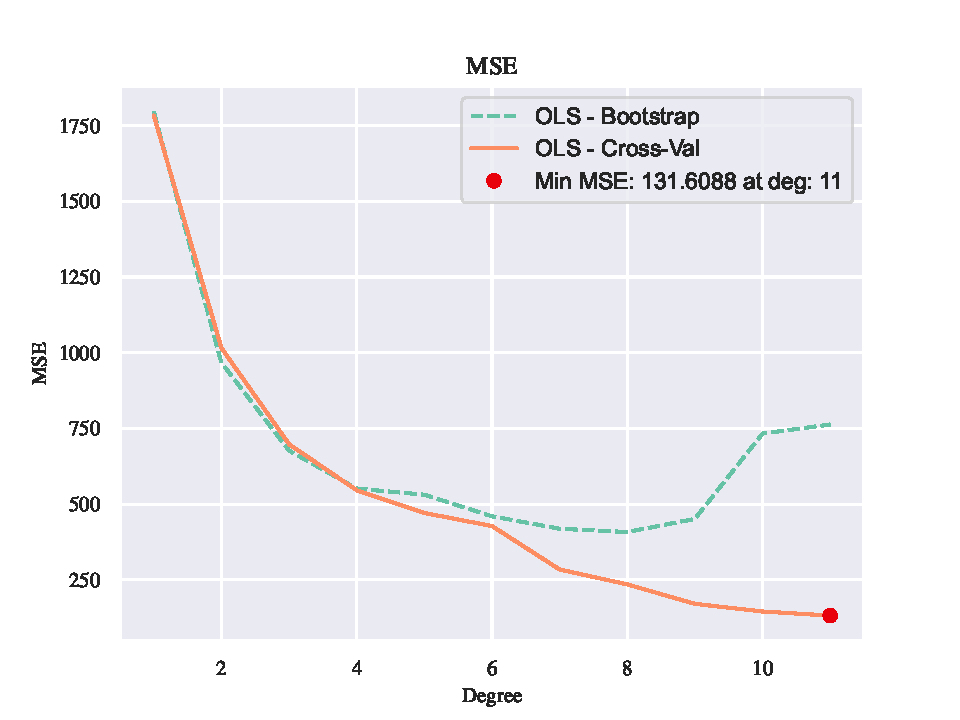
\includegraphics[width=1\linewidth]{project_1_alt/figures/figures_in_report/CV_BS_OLS_Terrain.pdf}
    \caption{MSE for three different models; ols-, ridge- and lasso regression against degree of complexity. All are trained with cross-validation.}
    \label{all_terrain_cv}
\end{figure}


In this section, the lasso- and ridge regression models are trained with their respective $\lambda$ values from Tab. \ref{tab:grid}. 

\begin{figure}[h!]
    \centering
    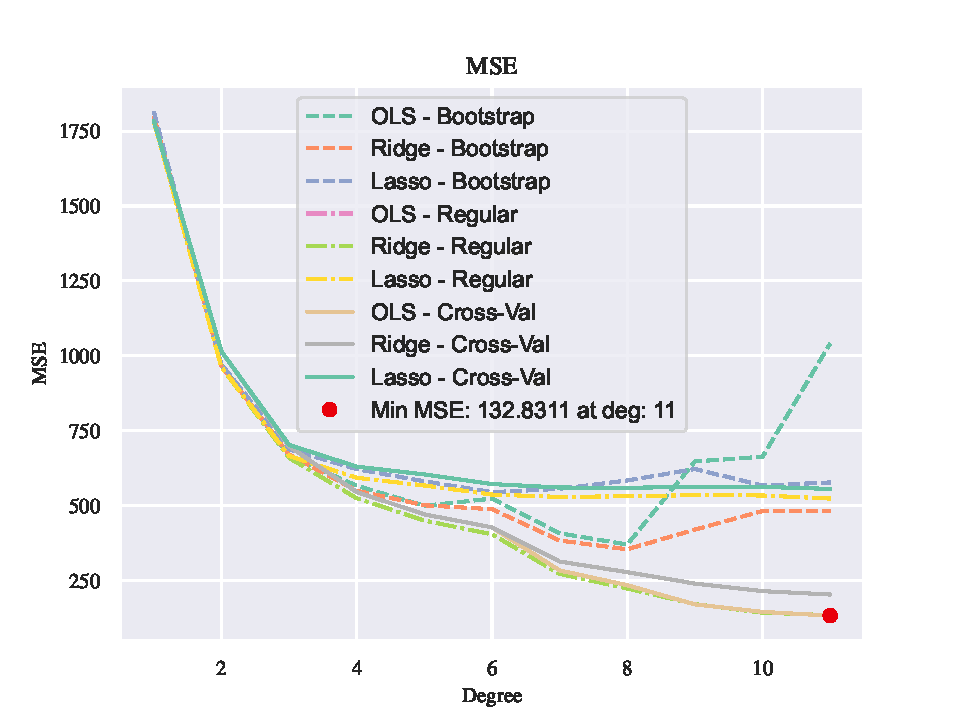
\includegraphics[width=1\linewidth]{project_1_alt/figures/figures_in_report/All_Terrain.pdf}
    \caption{MSE for ols-, ridge- and lasso regression against degree of complexity. Each model is trained three times; with no resampling, using cross-validation and lastly, using bootstrapping. The minimum is found for \mia{insert}}
    \label{all_terrain_OLS}
\end{figure}

In Fig. \ref{all_terrain_OLS} the error decreases for all three models as the degree of complexity increases. Ordinary least squares and lasso regression outperforms the rigde regression model. This might be due to \mia{smt}
When we use cross-validation to train all three models, ordinary least squares is the best performing model as shown in Fig. \ref{all_terrain_cv}. \mia{more}


\begin{figure}[h!]
    \centering
    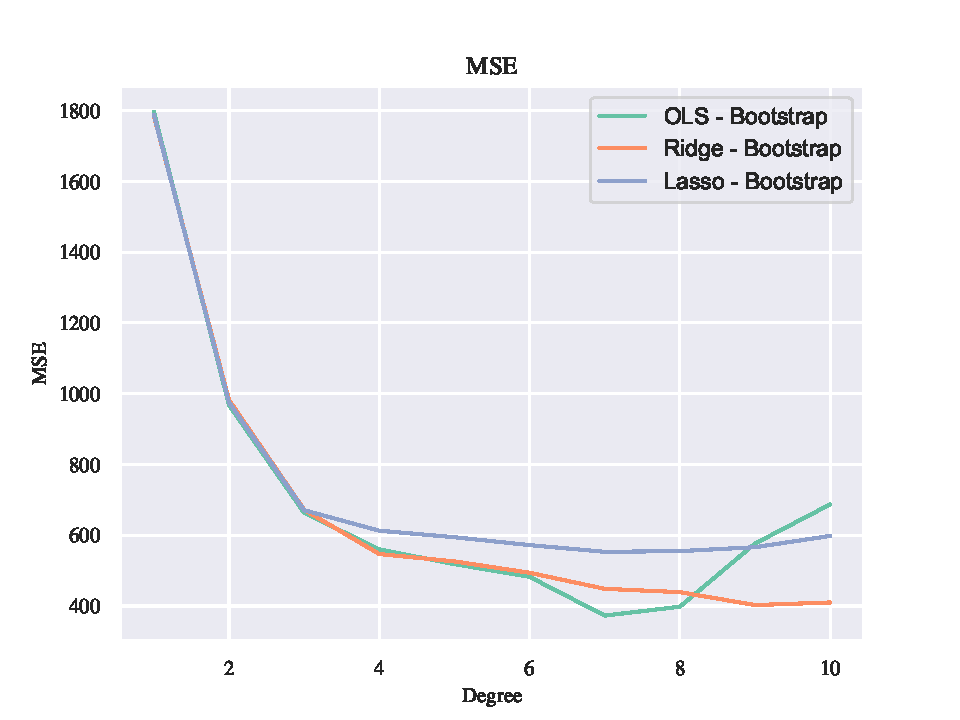
\includegraphics[width=1\linewidth]{project_1_alt/figures/figures_in_report/All_bootstrap_Terrain.pdf}
    \caption{MSE for three different models; ols-, ridge- and lasso regression against degree of complexity. All are trained with bootstrapping.}
    \label{all_terrain_bs}
\end{figure}

\mia{which one of the methods give the absolute lowest value for MSE $\rightarrow$ our best method yey}
\mia{discussion of which to trust the most}

\subsection{Overall discussion \mia{change this}}

Both the Franke function and the terrain data are chosen to have $41^2 = 1681$ data points. \mia{the impact of this + would maybe be natural to have way more points for the terrain data but we wanted to compare them?}

By including only a small section of the terrain data, the area in Fig. \ref{data:terrain} is quite rounded. 

\mia{discussion of whether it is even correct to compare the error measures (i.e. that the BS error measure is wrong) and that more data is utilized for the cv than for the bootstrap}

For the model trained with cross-validation, more data is utilized than for the one trained with bootstrap. In the ladder, we split into a training and a test data set, whereas cross-validation trains on the entire dataset. 

\mia{suggestions for further development: could implement bootstrap "corectly" (use different word) to have more data, non-linear methods}

Further work to do on this could include a different implementation of the bootstrap method. We could use the entire data set to draw bootstrap samples from. Then we would have to keep track of which samples were not included in the bootstrap sample and use these as the test set for the specific bootstrap model. This would allow us to use more data for training and improve the model. 

Furthermore, it is interesting to discuss whether linear models are sufficient for these kinds of problems or not. \mia{continue}